\documentclass[color=usenames,dvipsnames]{beamer}\usepackage[]{graphicx}\usepackage[]{color}
% maxwidth is the original width if it is less than linewidth
% otherwise use linewidth (to make sure the graphics do not exceed the margin)
\makeatletter
\def\maxwidth{ %
  \ifdim\Gin@nat@width>\linewidth
    \linewidth
  \else
    \Gin@nat@width
  \fi
}
\makeatother

\definecolor{fgcolor}{rgb}{0, 0, 0}
\newcommand{\hlnum}[1]{\textcolor[rgb]{0.69,0.494,0}{#1}}%
\newcommand{\hlstr}[1]{\textcolor[rgb]{0.749,0.012,0.012}{#1}}%
\newcommand{\hlcom}[1]{\textcolor[rgb]{0.514,0.506,0.514}{\textit{#1}}}%
\newcommand{\hlopt}[1]{\textcolor[rgb]{0,0,0}{#1}}%
\newcommand{\hlstd}[1]{\textcolor[rgb]{0,0,0}{#1}}%
\newcommand{\hlkwa}[1]{\textcolor[rgb]{0,0,0}{\textbf{#1}}}%
\newcommand{\hlkwb}[1]{\textcolor[rgb]{0,0.341,0.682}{#1}}%
\newcommand{\hlkwc}[1]{\textcolor[rgb]{0,0,0}{\textbf{#1}}}%
\newcommand{\hlkwd}[1]{\textcolor[rgb]{0.004,0.004,0.506}{#1}}%
\let\hlipl\hlkwb

\usepackage{framed}
\makeatletter
\newenvironment{kframe}{%
 \def\at@end@of@kframe{}%
 \ifinner\ifhmode%
  \def\at@end@of@kframe{\end{minipage}}%
  \begin{minipage}{\columnwidth}%
 \fi\fi%
 \def\FrameCommand##1{\hskip\@totalleftmargin \hskip-\fboxsep
 \colorbox{shadecolor}{##1}\hskip-\fboxsep
     % There is no \\@totalrightmargin, so:
     \hskip-\linewidth \hskip-\@totalleftmargin \hskip\columnwidth}%
 \MakeFramed {\advance\hsize-\width
   \@totalleftmargin\z@ \linewidth\hsize
   \@setminipage}}%
 {\par\unskip\endMakeFramed%
 \at@end@of@kframe}
\makeatother

\definecolor{shadecolor}{rgb}{.97, .97, .97}
\definecolor{messagecolor}{rgb}{0, 0, 0}
\definecolor{warningcolor}{rgb}{1, 0, 1}
\definecolor{errorcolor}{rgb}{1, 0, 0}
\newenvironment{knitrout}{}{} % an empty environment to be redefined in TeX

\usepackage{alltt}
%\documentclass[color=usenames,dvipsnames,handout]{beamer}

\usepackage[roman]{../lectures}


\hypersetup{pdfpagemode=UseNone,pdfstartview={FitV}}

\title{Lecture 1 -- Introduction to }
\author{Richard Chandler}


% Load function to compile and open PDF


% Compile and open PDF





%<<knitr-setup,include=FALSE,purl=FALSE>>=
%##opts_chunk$set(comment=NA)
%@


%% New command for inline code that isn't to be evaluated
\definecolor{inlinecolor}{rgb}{0.878, 0.918, 0.933}
\newcommand{\inr}[1]{\colorbox{inlinecolor}{\texttt{#1}}}
\IfFileExists{upquote.sty}{\usepackage{upquote}}{}
\begin{document}


\begin{frame}[plain]
  \LARGE
%  \maketitle
  \centering
  {\huge %\bf
    Lecture 1 -- Overview} \\
  {\color{default} \rule{\textwidth}{0.1pt}}
  \vfill
  \large
  WILD(FISH) 8390 \\
  Estimation of Fish and Wildlife Population Parameters \\
  \vfill
  Richard Chandler \\
  University of Georgia
\end{frame}



\section{Overview}


\begin{frame}[plain]
  \frametitle{Today's Topics}
  \Large
  \only<1>{\tableofcontents}
  \only<2 | handout:0>{\tableofcontents[currentsection]}
\end{frame}



\begin{frame}[fragile]
  \frametitle{Overview}
  {\Large Themes}
  \begin{itemize}
    \item<1-> We need models to:
      \begin{itemize}[<1->]
        \item Evaluate hypotheses
        \item Make predictions
        \item Forecast future outcomes
        \item Inform management decisions
      \end{itemize}
    \item<2-> Until recently, models were mainly used in theoretical settings
    \item<3-> New statistical tools let us confront models with data
    \item<4-> Hierarchical models allow us to describe 
      conditional ecological and observation processes
    \item<5-> Before we even collect our data, we should:
      \begin{itemize}
        \item Write down hypotheses about the processes that are likely to give 
          rise to our observations
        \item Formalize these processes as statistical models
      \end{itemize}
  \end{itemize}
\end{frame}




\begin{frame}
  \frametitle{Classical models of population dynamics}
  Classical models of population dynamics provide a critical reference
  for developing custom models for specific populations and
  applications. \\
  \pause
  \vfill
  A working knowledge of the following models is important:
  \begin{itemize}
    \item Exponential growth
    \item Logistic growth
    \item Stage-structured matrix models
    \item Metapopulation models
  \end{itemize}
\end{frame}


\begin{frame}
  \frametitle{Classical statistical models}
  Classical statistical models are equally important. \\
  \pause
  \vfill
  You should be familiar with:
  \begin{itemize}
    \item Linear models (including the various *NOVAs)
    \item Generalized linear models (eg, logistic regression)
    \item Generalized linear mixed effects models
  \end{itemize}
\end{frame}



\begin{frame}
  \LARGE 
  \centering
  How do we bridge the gap between theoretical models and statistical 
  models?  \\
\end{frame}


\section{Examples}


\subsection{Chiricahua Leopard Frogs}


\begin{frame}
  \frametitle{Example I -- Chiricahua Leopard Frogs}
  \begin{columns}
    \setlength\fboxsep{0pt}
    \begin{column}{0.5\textwidth}
      \small
      \vbox to .8\textheight{
        Sites are discrete habitat patches \\
        \vfill
        Surrounding landscape is suitable for movement but not
        reproduction \\
        \vfill
        Data are binary detection data \\
        \vfill
        \fbox{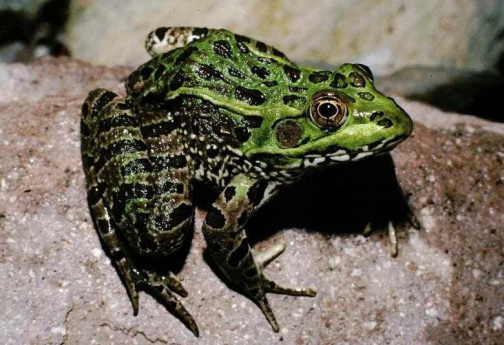
\includegraphics[width=\textwidth]{figs/lich}}
      }
    \end{column}
    \begin{column}{0.5\textwidth}
      \fbox{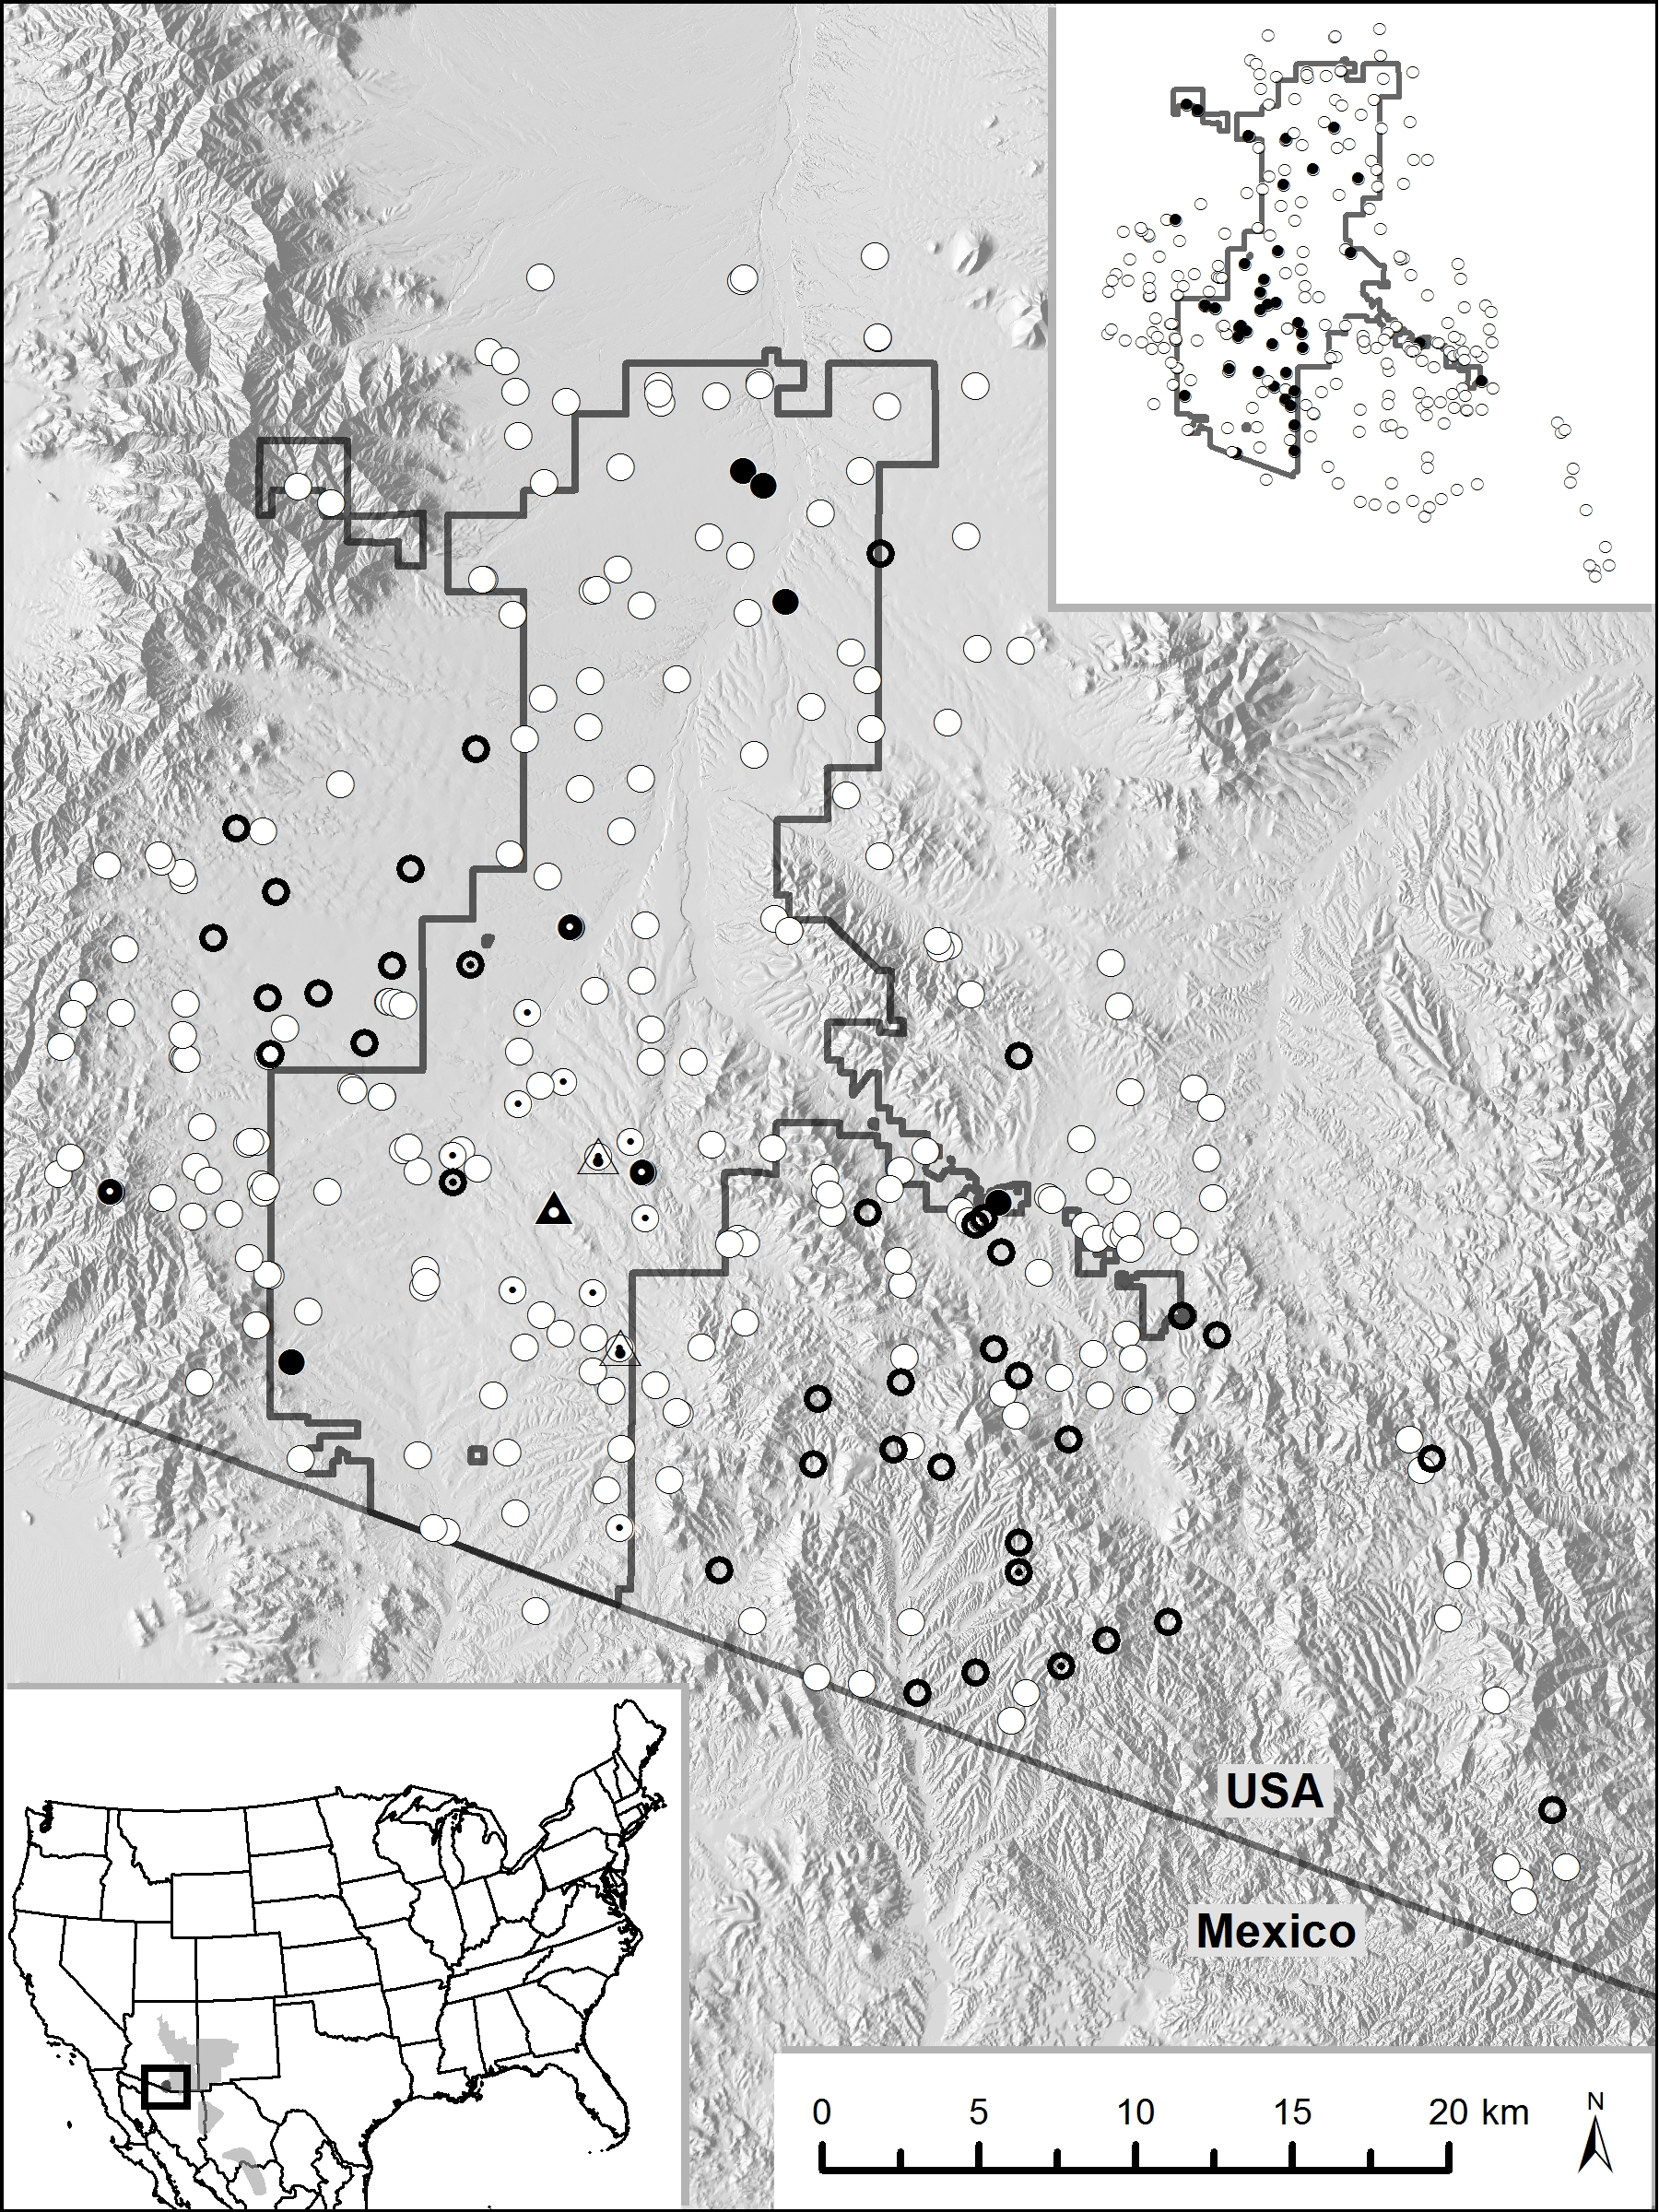
\includegraphics[width=\textwidth]{figs/lich-dist}}
    \end{column}
  \end{columns}
\end{frame}



\begin{frame}
  \frametitle{Metapopulation ecology}
  \begin{columns}
    \setlength\fboxsep{0pt}
    \begin{column}{0.6\textwidth}
      \small
      \vbox to 0.7\textheight{
        Large body of theory \\
        % \pause
        \vfill
        \uncover<2->{One branch of metapopulation theory focuses on
          distance-dependent colonization and extinction processes} \\
        % \pause
        \vfill
        \uncover<3->{If we know the patch coordinates and we have data from
          multiple sites and multiple time periods, we can fit the
          models} \\
      }
    \end{column}
    \begin{column}{0.4\textwidth}
      \fbox{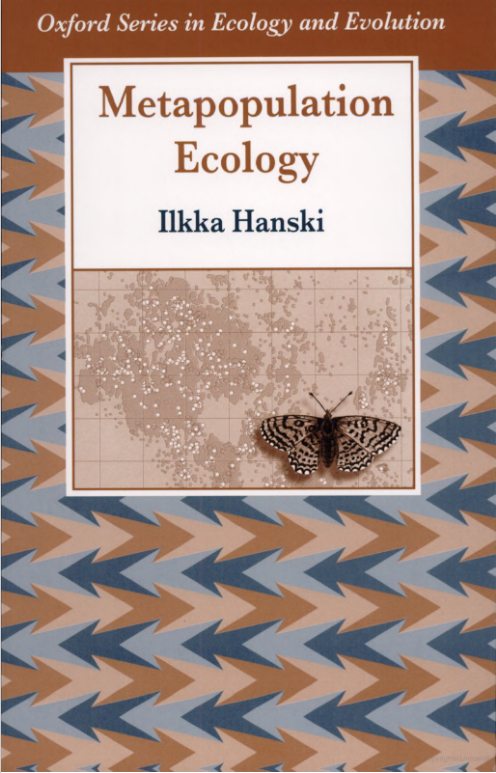
\includegraphics[width=\textwidth]{figs/HanskiBookCover}}
    \end{column}
  \end{columns}
\end{frame}



\begin{frame}
  \frametitle{Recovery Plan}
  \begin{columns}
    \wide
    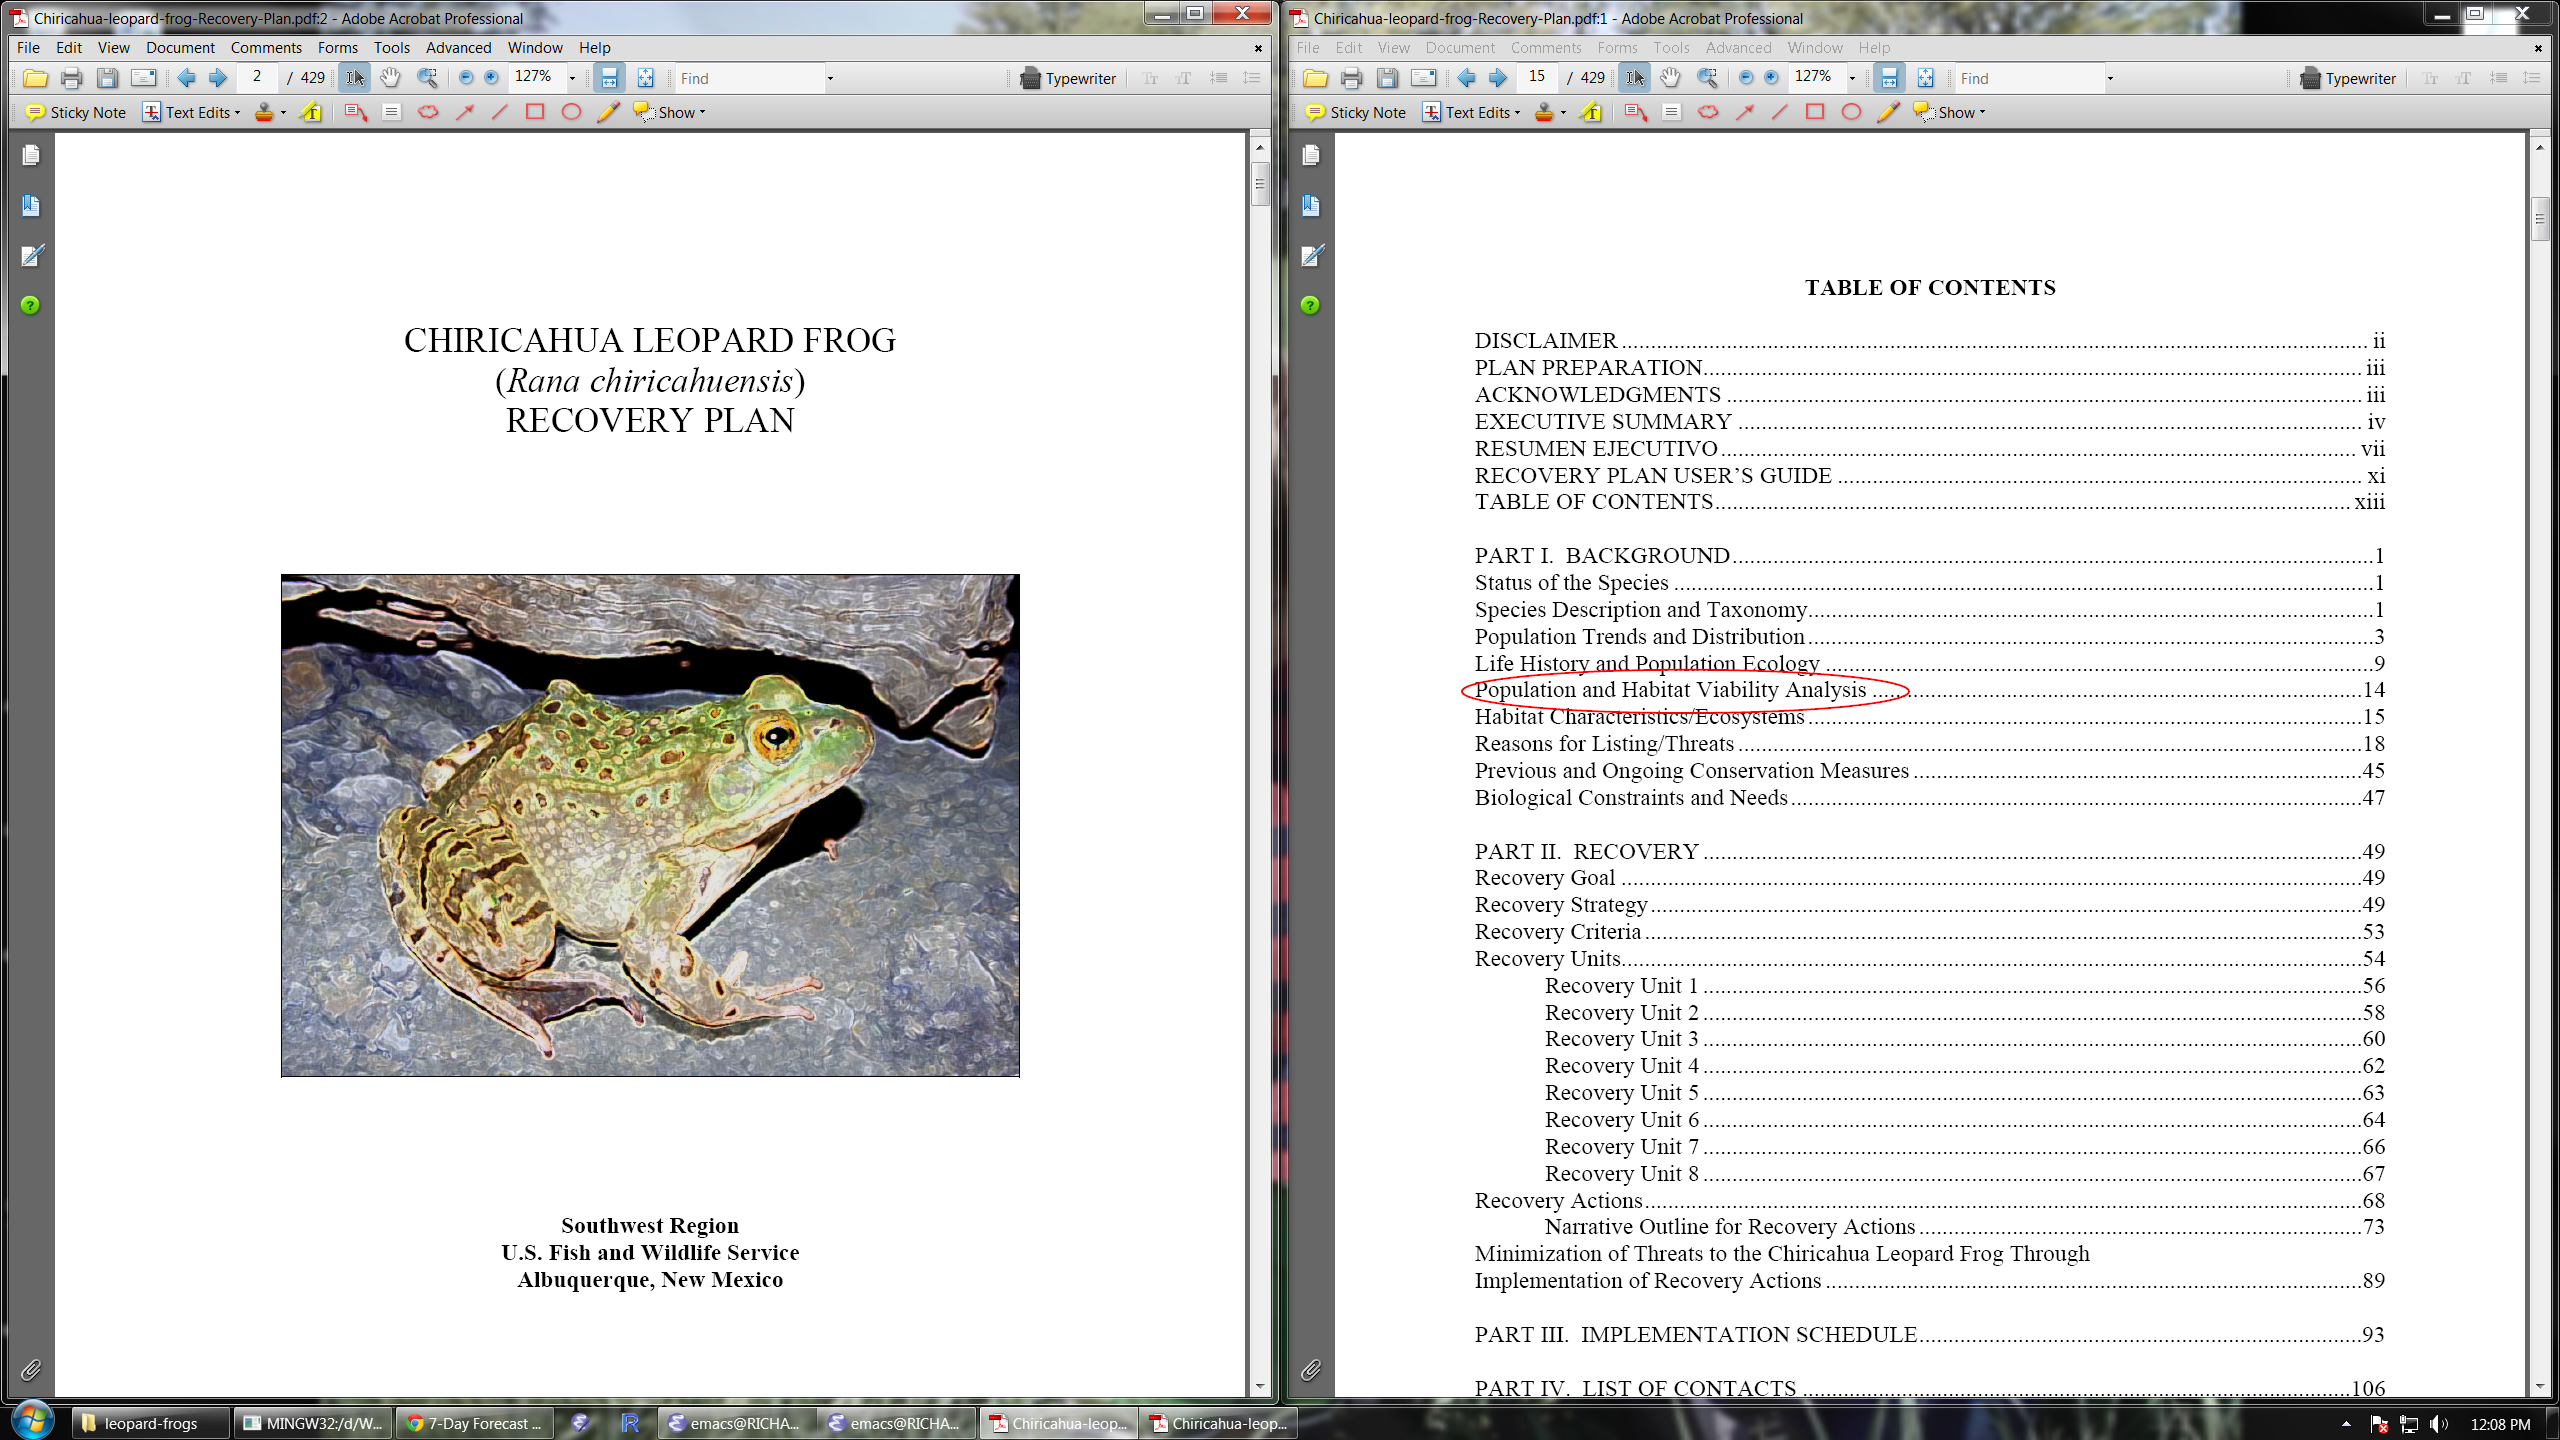
\includegraphics[width=\textwidth]{figs/lich-recovery-plan}
  \end{columns}
\end{frame}



\begin{frame}
  \frametitle{Estimated extinction risk\footnote{\scriptsize Howell et al. (2020, Ecological Applications)}}
  \begin{columns}
    \begin{column}{0.6\textwidth}
      \begin{itemize}%[<+->]
      \item<1-> Metapopulation models fit to the detection
        data 
      \item[]
      \item<2-> Extinction probability estimated to be 2\% by 2100
      \item[]
      \item<3-> What can be done about it?
        \begin{itemize}
        \item<4-> Control predators
        \item<4-> Increase hydroperiod in existing wetlands
        \item<4-> Create new wetlands\dots
%        \item<6-> \dots but where?
        \end{itemize}
      \end{itemize}
    \end{column}
    \begin{column}{0.38\textwidth}
      \begin{center}
%        \includegraphics[width=0.4\textwidth]{figs/extinction3}
        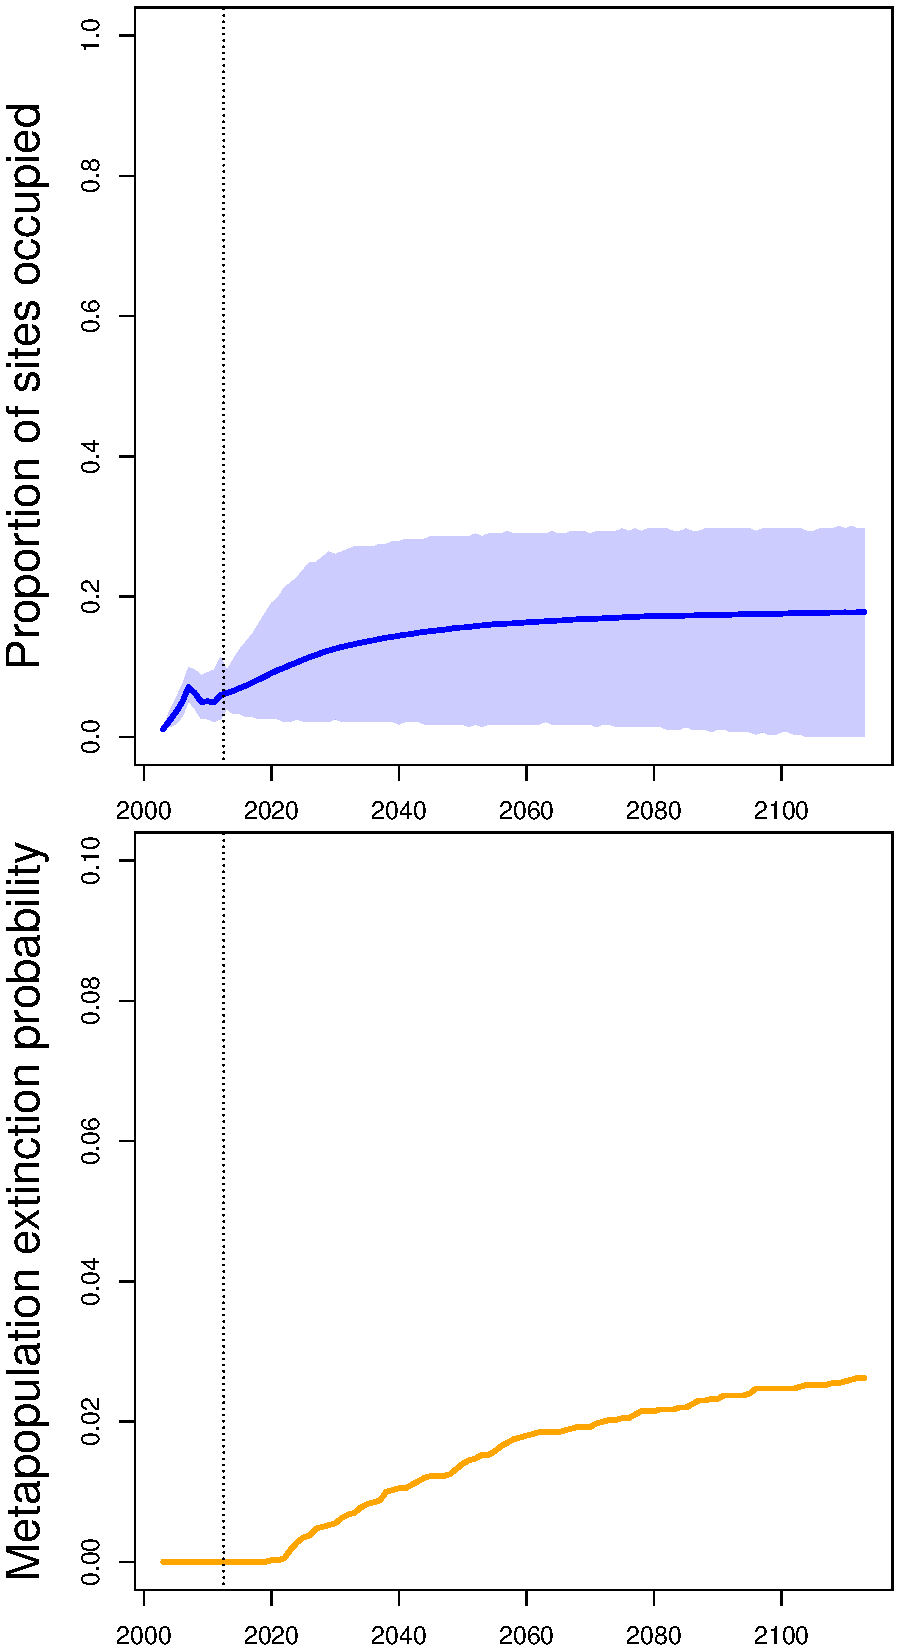
\includegraphics[width=\textwidth]{figs/proj-ext-JAPPL}
      \end{center}
    \end{column}
  \end{columns}
  
\end{frame}




\begin{frame}
  \frametitle{Extinction risk}
  \begin{center}
    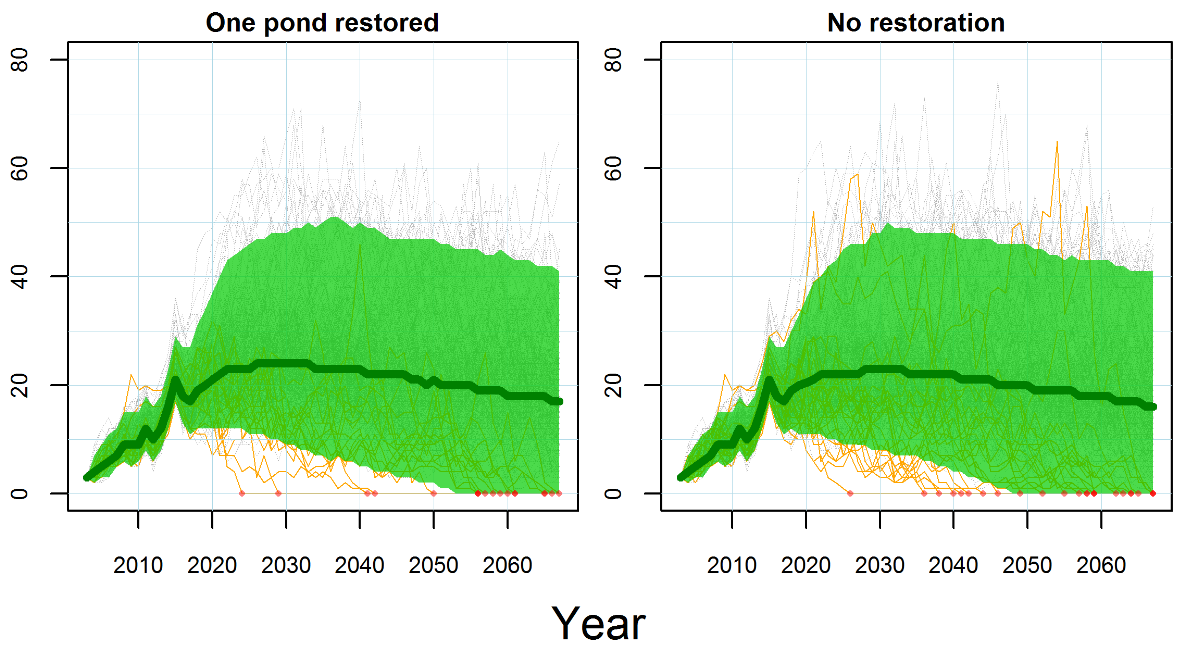
\includegraphics[width=\textwidth]{figs/lich-forecasts}
  \end{center}
\end{frame}



\begin{frame}
  \frametitle{Colonization Probability Maps}
  \begin{center}
    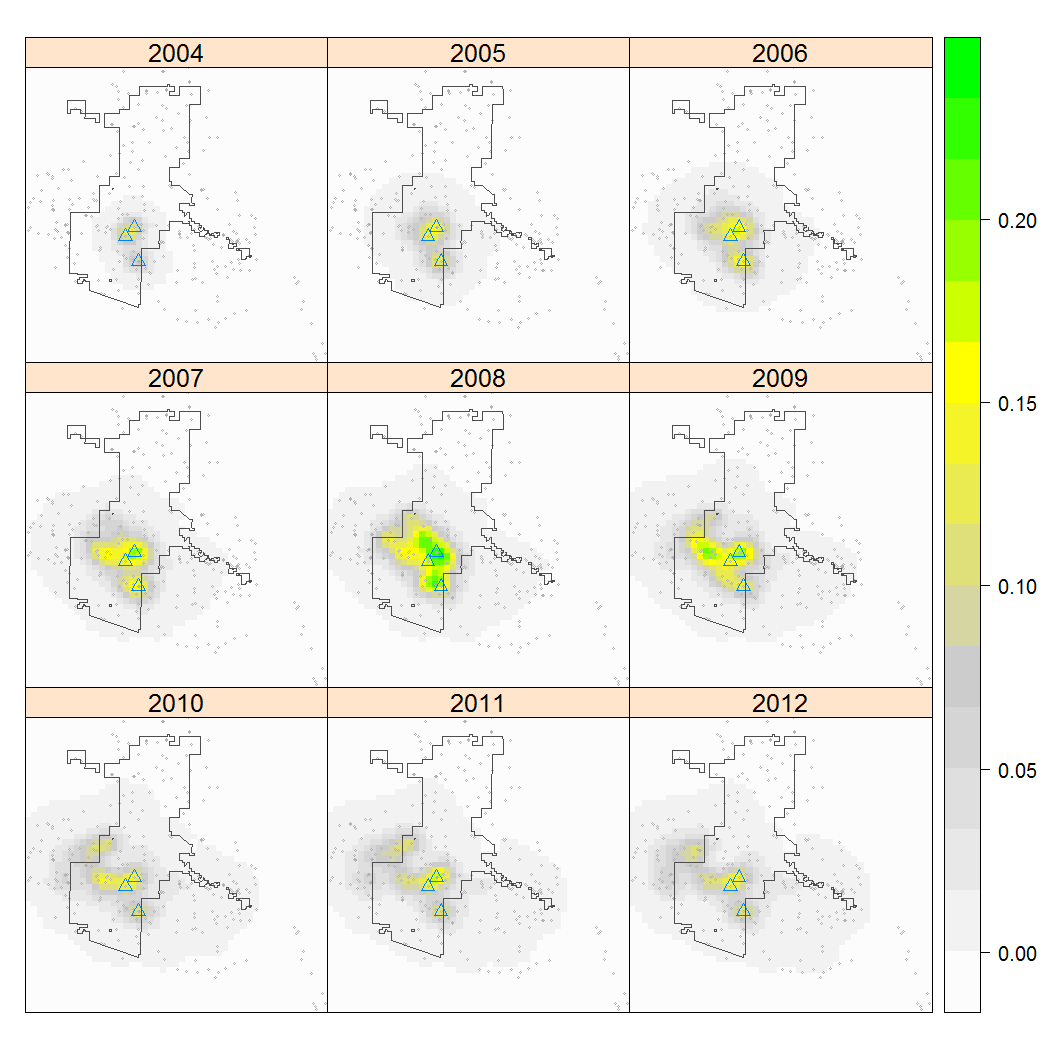
\includegraphics[width=0.7\textwidth]{figs/colMap1-9nohill}
  \end{center}
\end{frame}




\subsection{Central Georgia Black Bears}


\begin{frame}
  \frametitle{Example II -- Central Georgia Black Bears}
  \begin{columns}
    \begin{column}{0.5\textwidth}
      \vbox to 0.6\textheight{
        Genetically isolated population near Macon \\
        \vfill
        Impacts of hunting had not been evaluated \\
        \vfill
        Studied using noninvasive genetic mark-recapture \\
        \vfill
        Hair snares and genotyping yielded individual-level encounter
        histories \\
      }
    \end{column}
    \begin{column}{0.5\textwidth}
      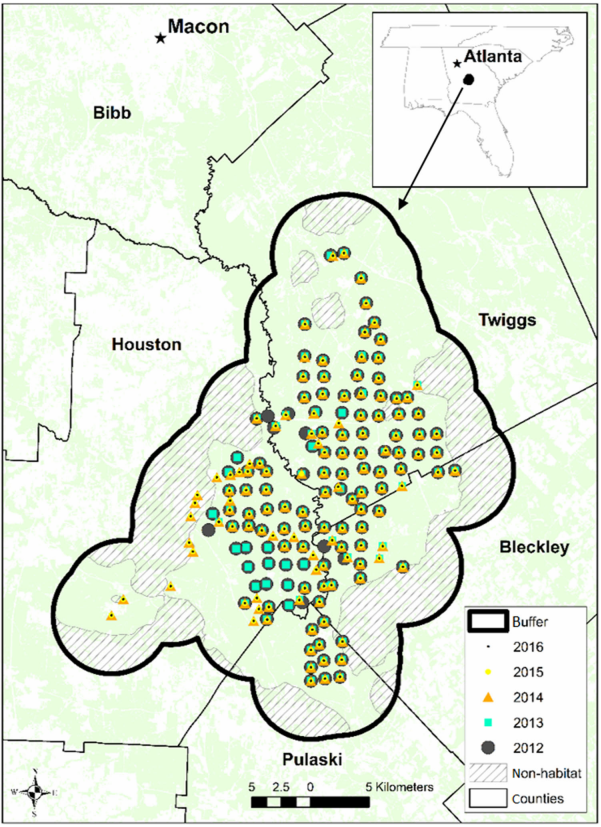
\includegraphics[width=\textwidth]{figs/GA_bear_map} \\
    \end{column}
  \end{columns}
\end{frame}



\begin{frame}
  \frametitle{Harvest theory}
  \begin{columns}
    \setlength\fboxsep{0pt}
    \begin{column}{0.6\textwidth}
      \small
      \vbox to 0.6\textheight{
        \uncover<1->{Theory goes back about a century} \\
        \vfill
        \uncover<2->{Much of it focuses on the importance of density dependence} \\
        \vfill
        \uncover<3->{Think back to ``maximum sustainable yield''}
      }
    \end{column}
    \begin{column}{0.4\textwidth}
      \fbox{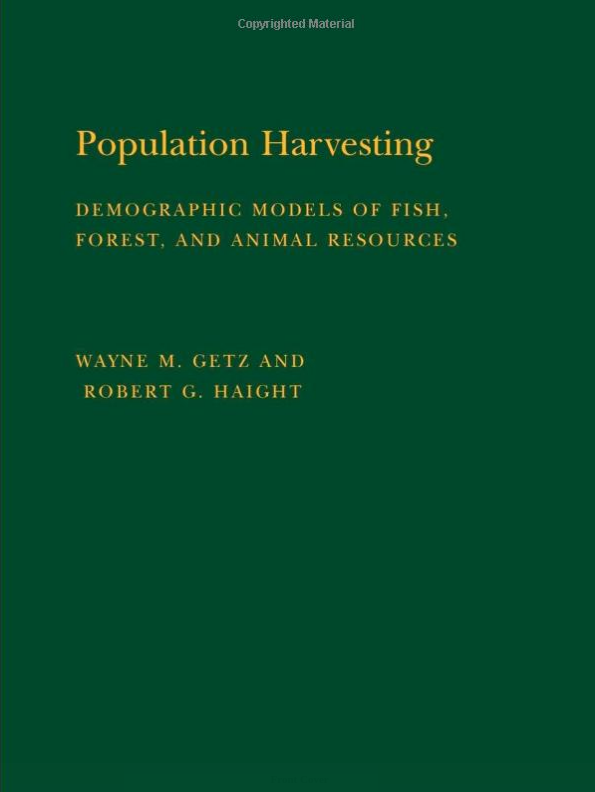
\includegraphics[width=\textwidth]{figs/GetzHaightBookCover}}
    \end{column}
  \end{columns}
\end{frame}



\begin{frame}
  \frametitle{Central Georgia Black Bears}
  Female-based population model revealed population
  growth\footnote{Hooker et al. (2020, Journal of Wildlife Management)} \\
  \centering
  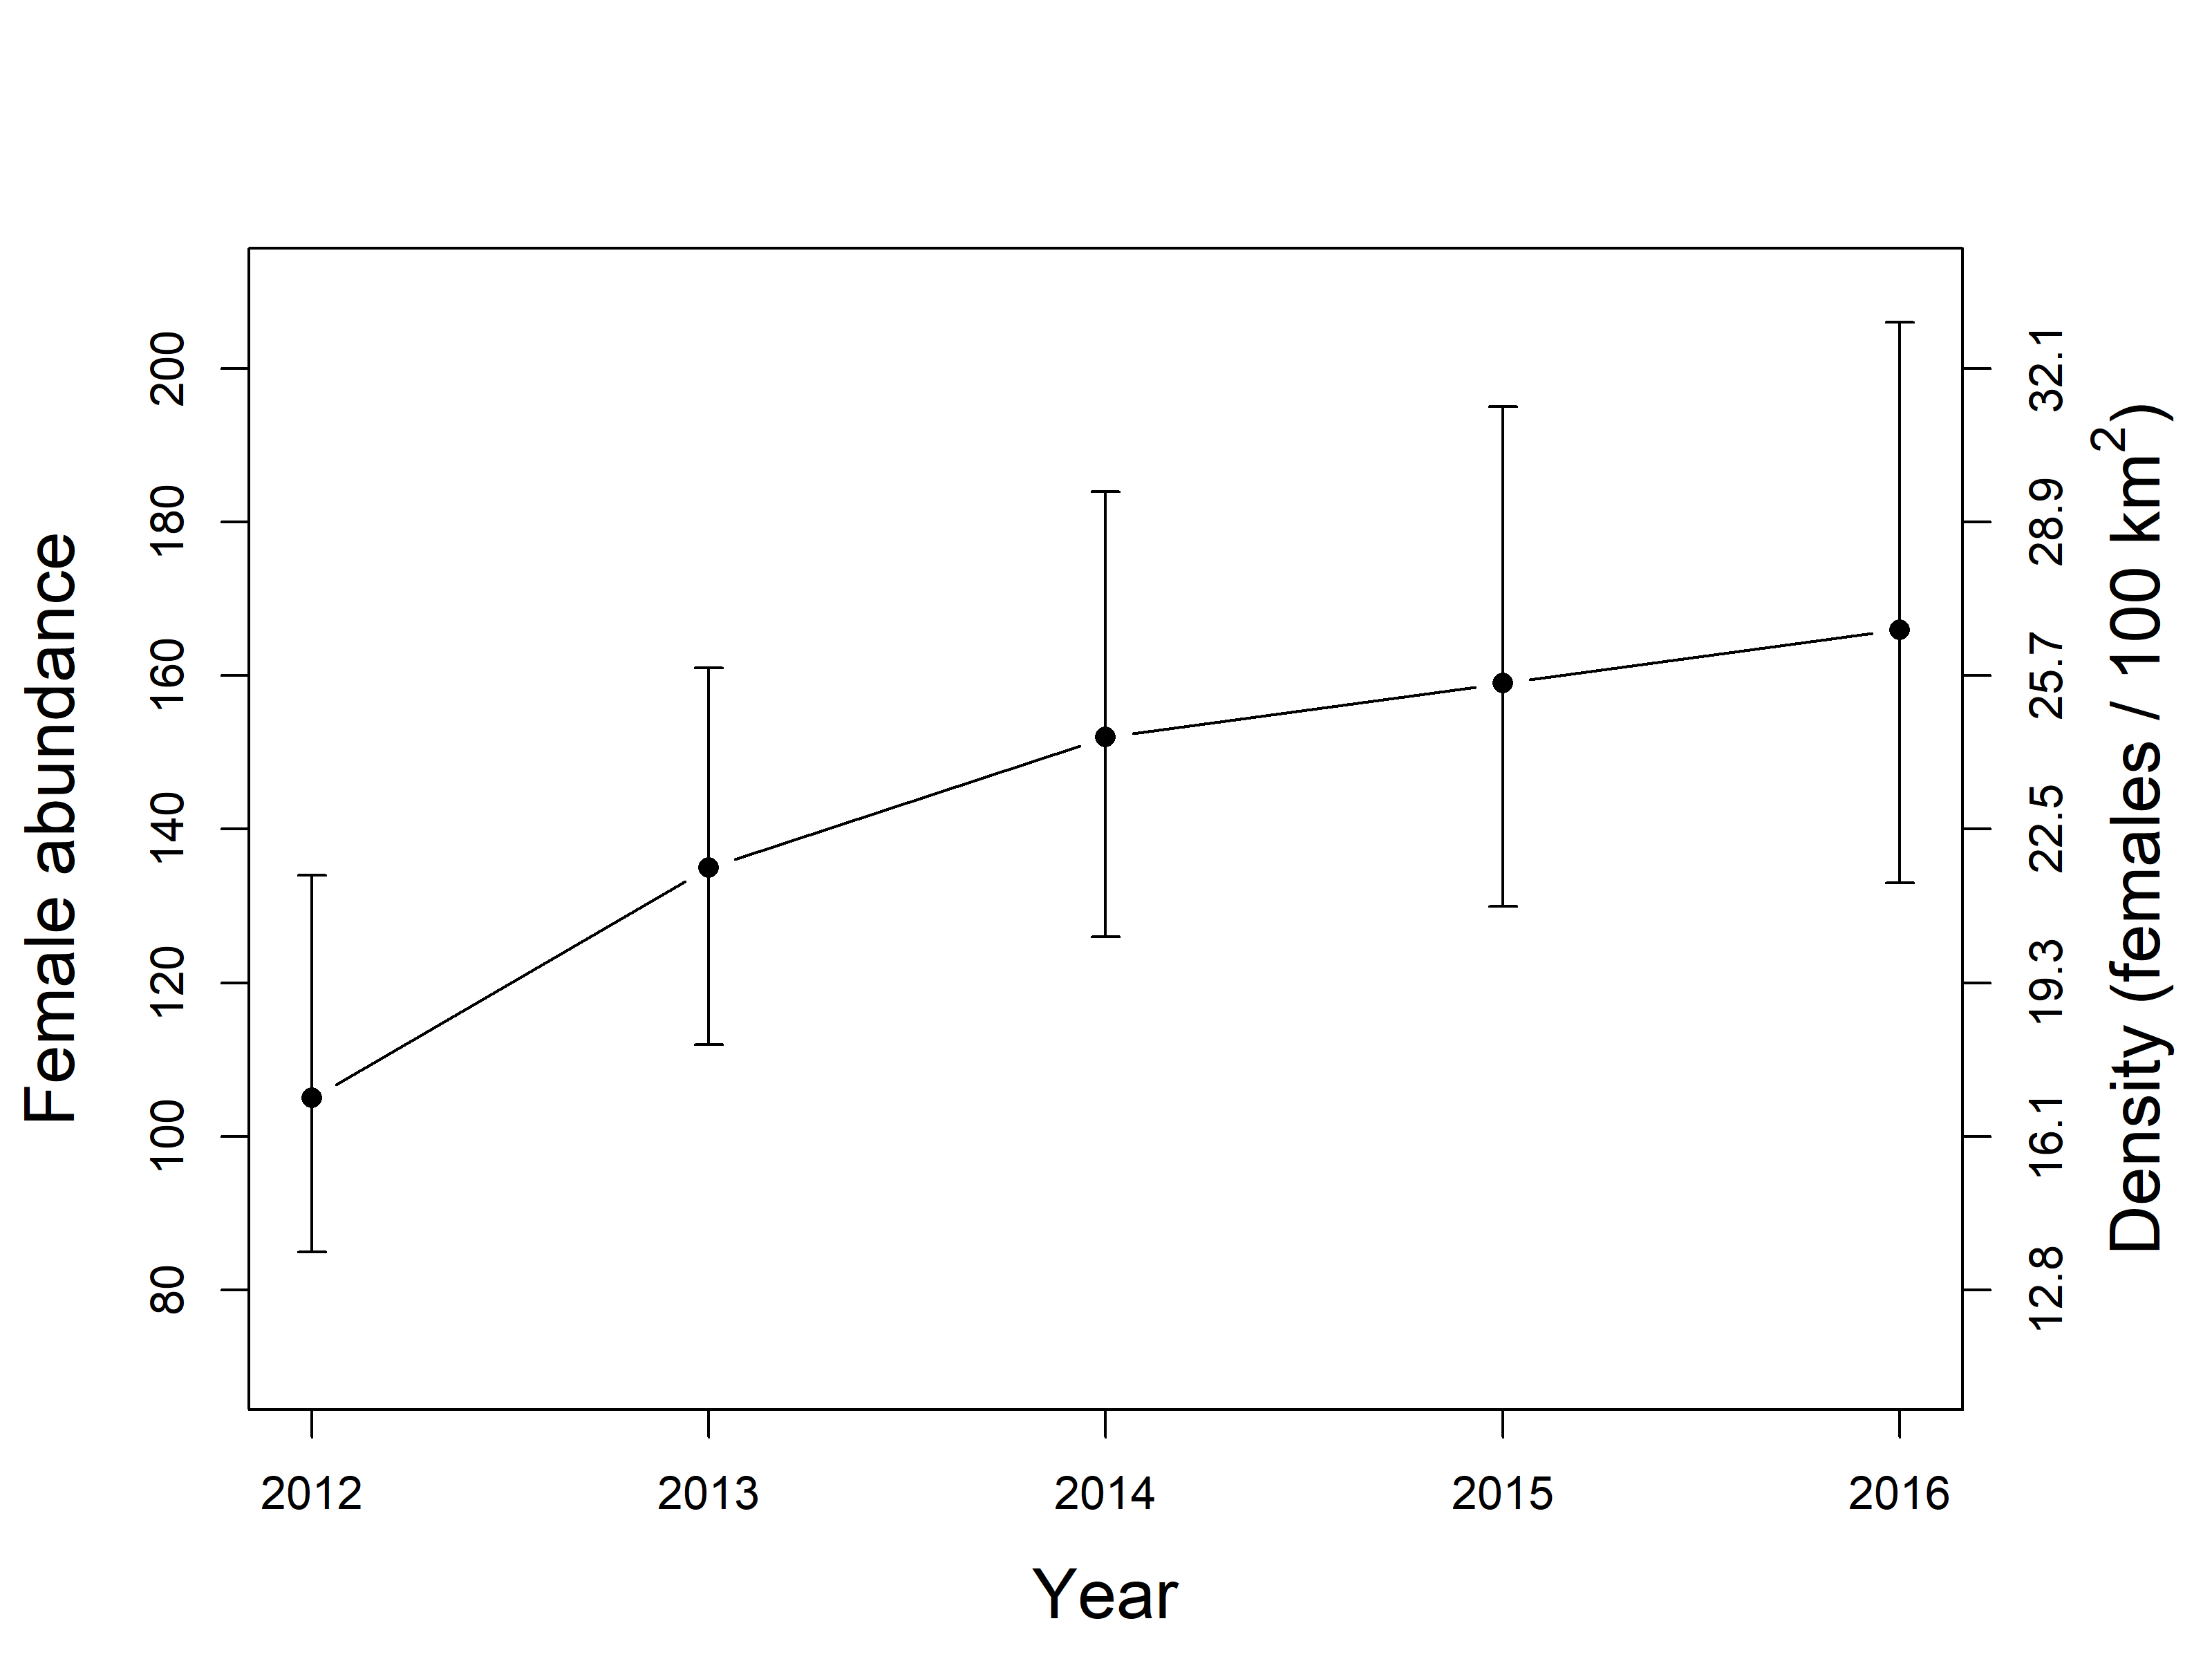
\includegraphics[width=0.9\textwidth,trim=0mm 0mm 0mm 10mm,clip]{figs/fig-5_abundance} \\
\end{frame}


\begin{frame}
  \frametitle{Central Georgia Black Bears}
  Population regulated by density-dependent recruitment \\
  \vfill
  \centering
  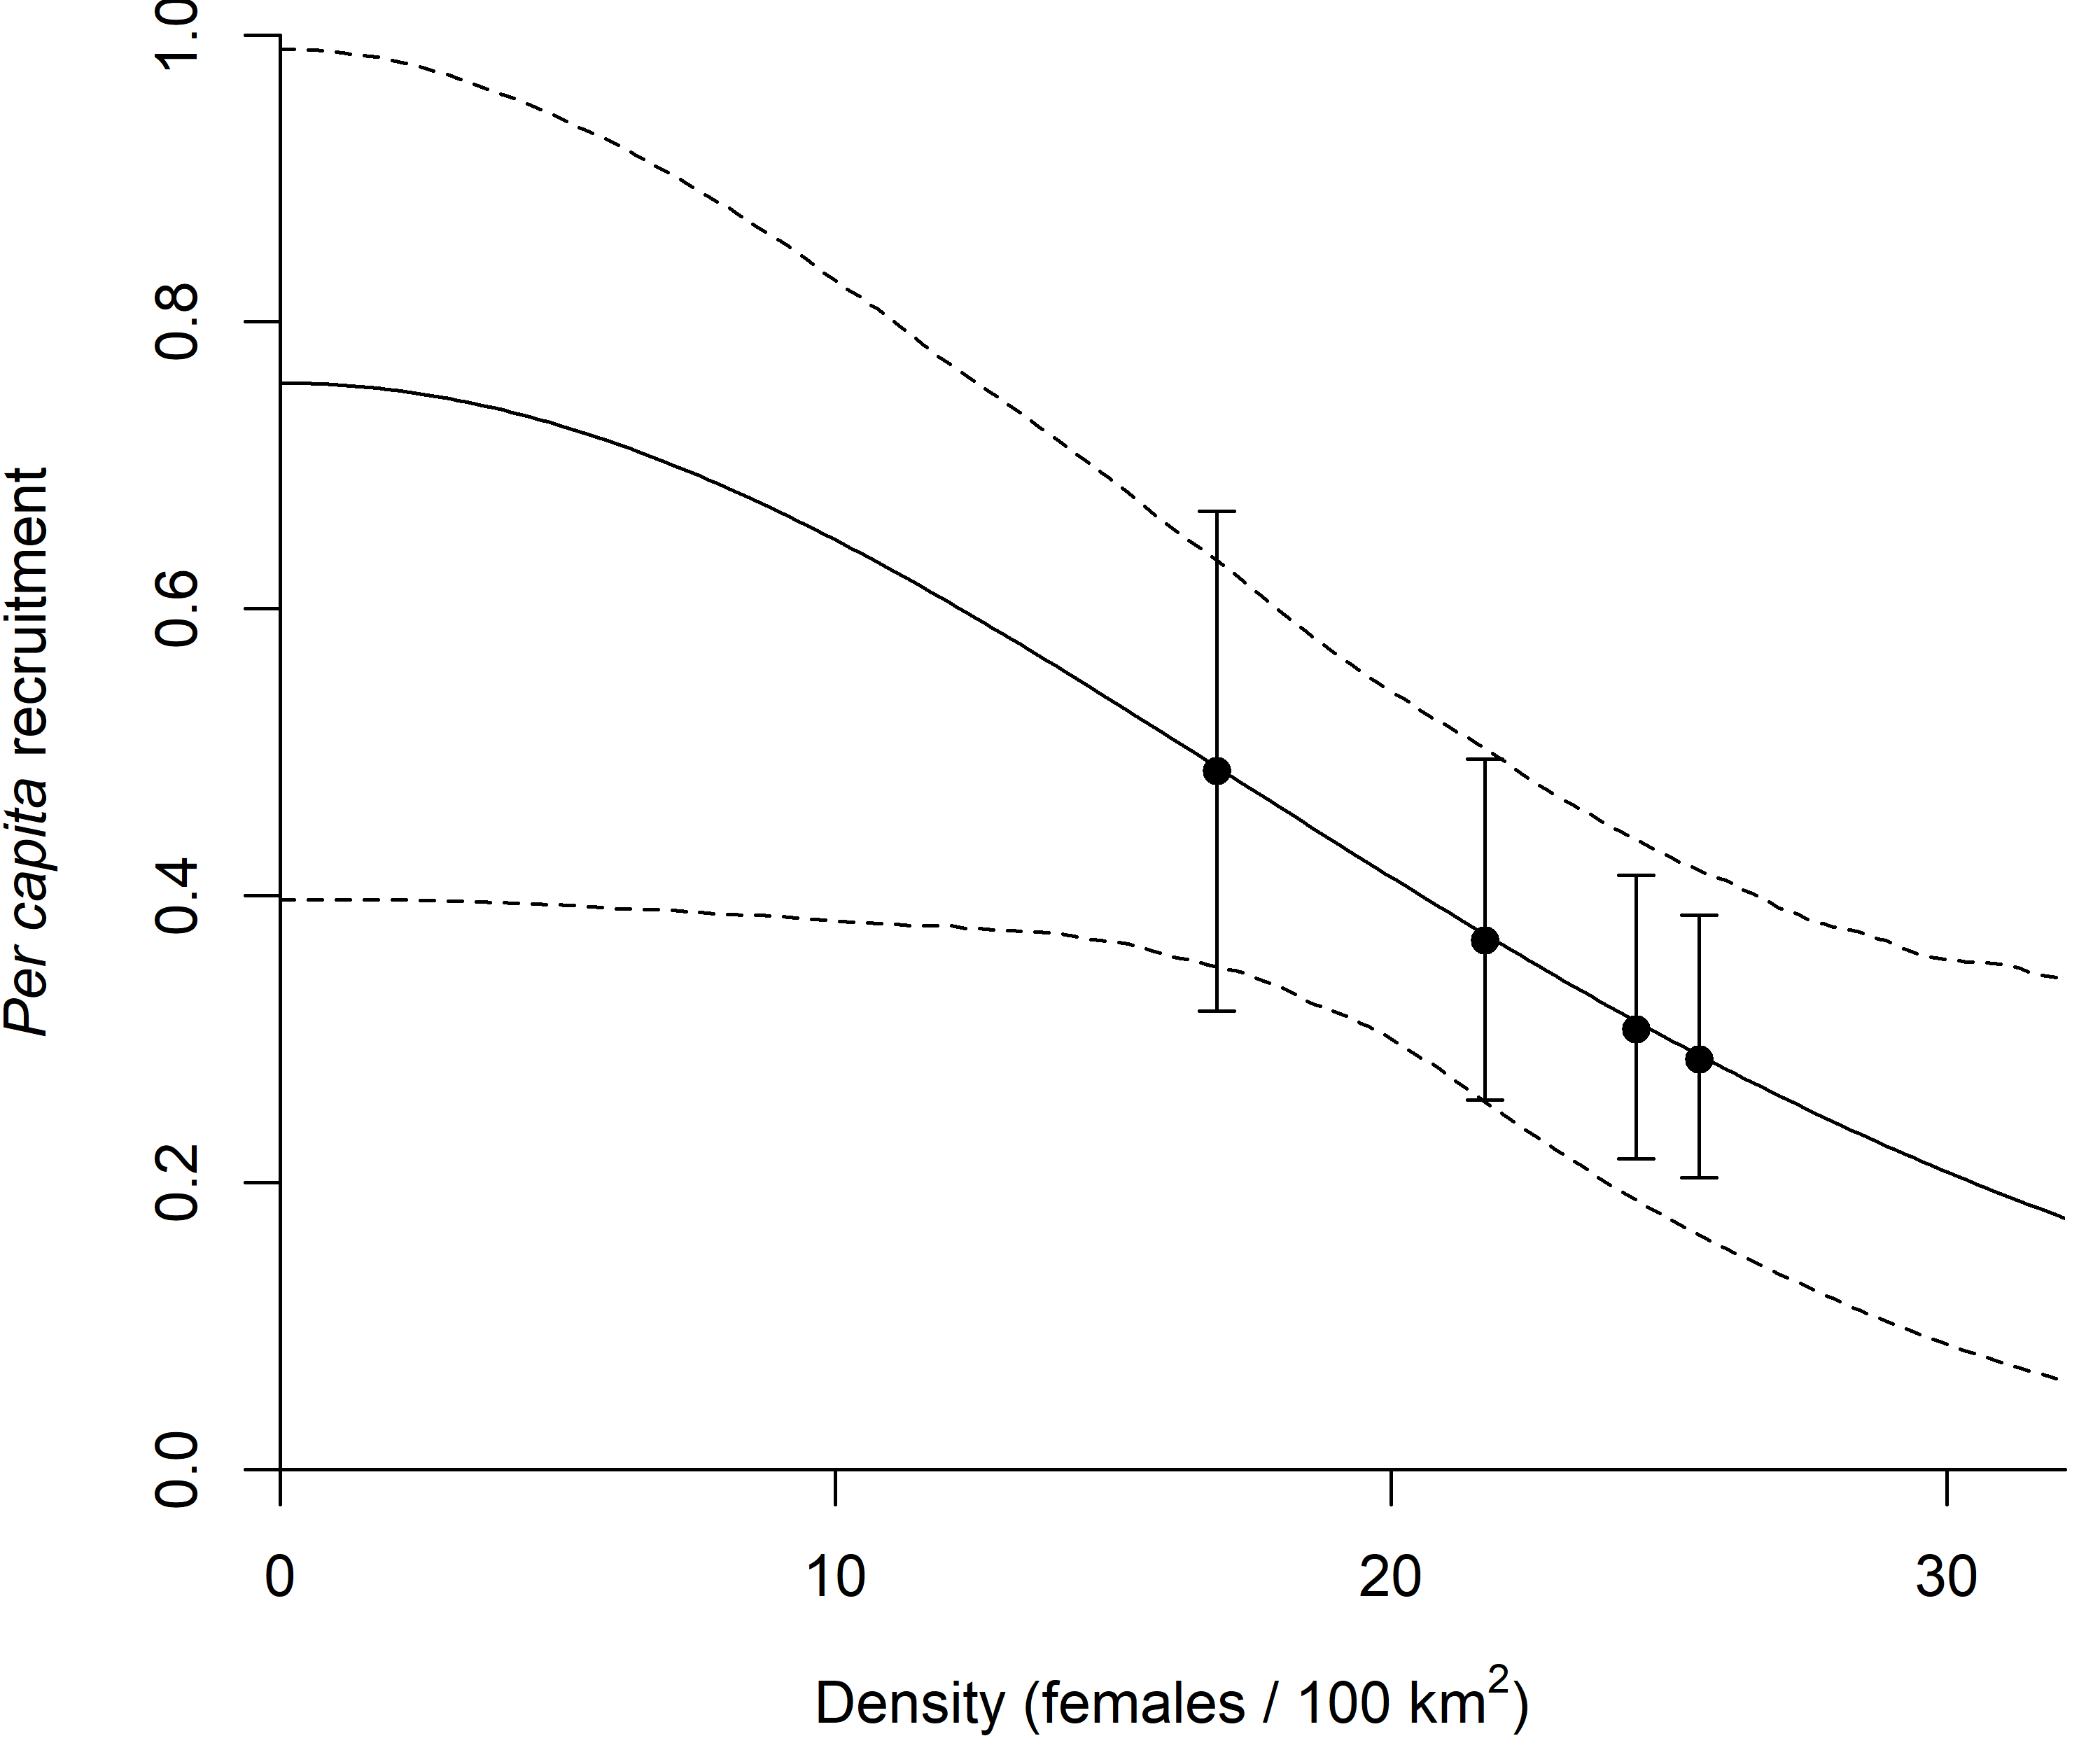
\includegraphics[width=0.7\textwidth]{figs/fig-3_dd-recruitment} \\
\end{frame}


\begin{frame}
  \frametitle{Central Georgia Black Bears}
  Extinction risk low unless harvest increases by $>$10 females/year \\
  \vfill
  \centering
  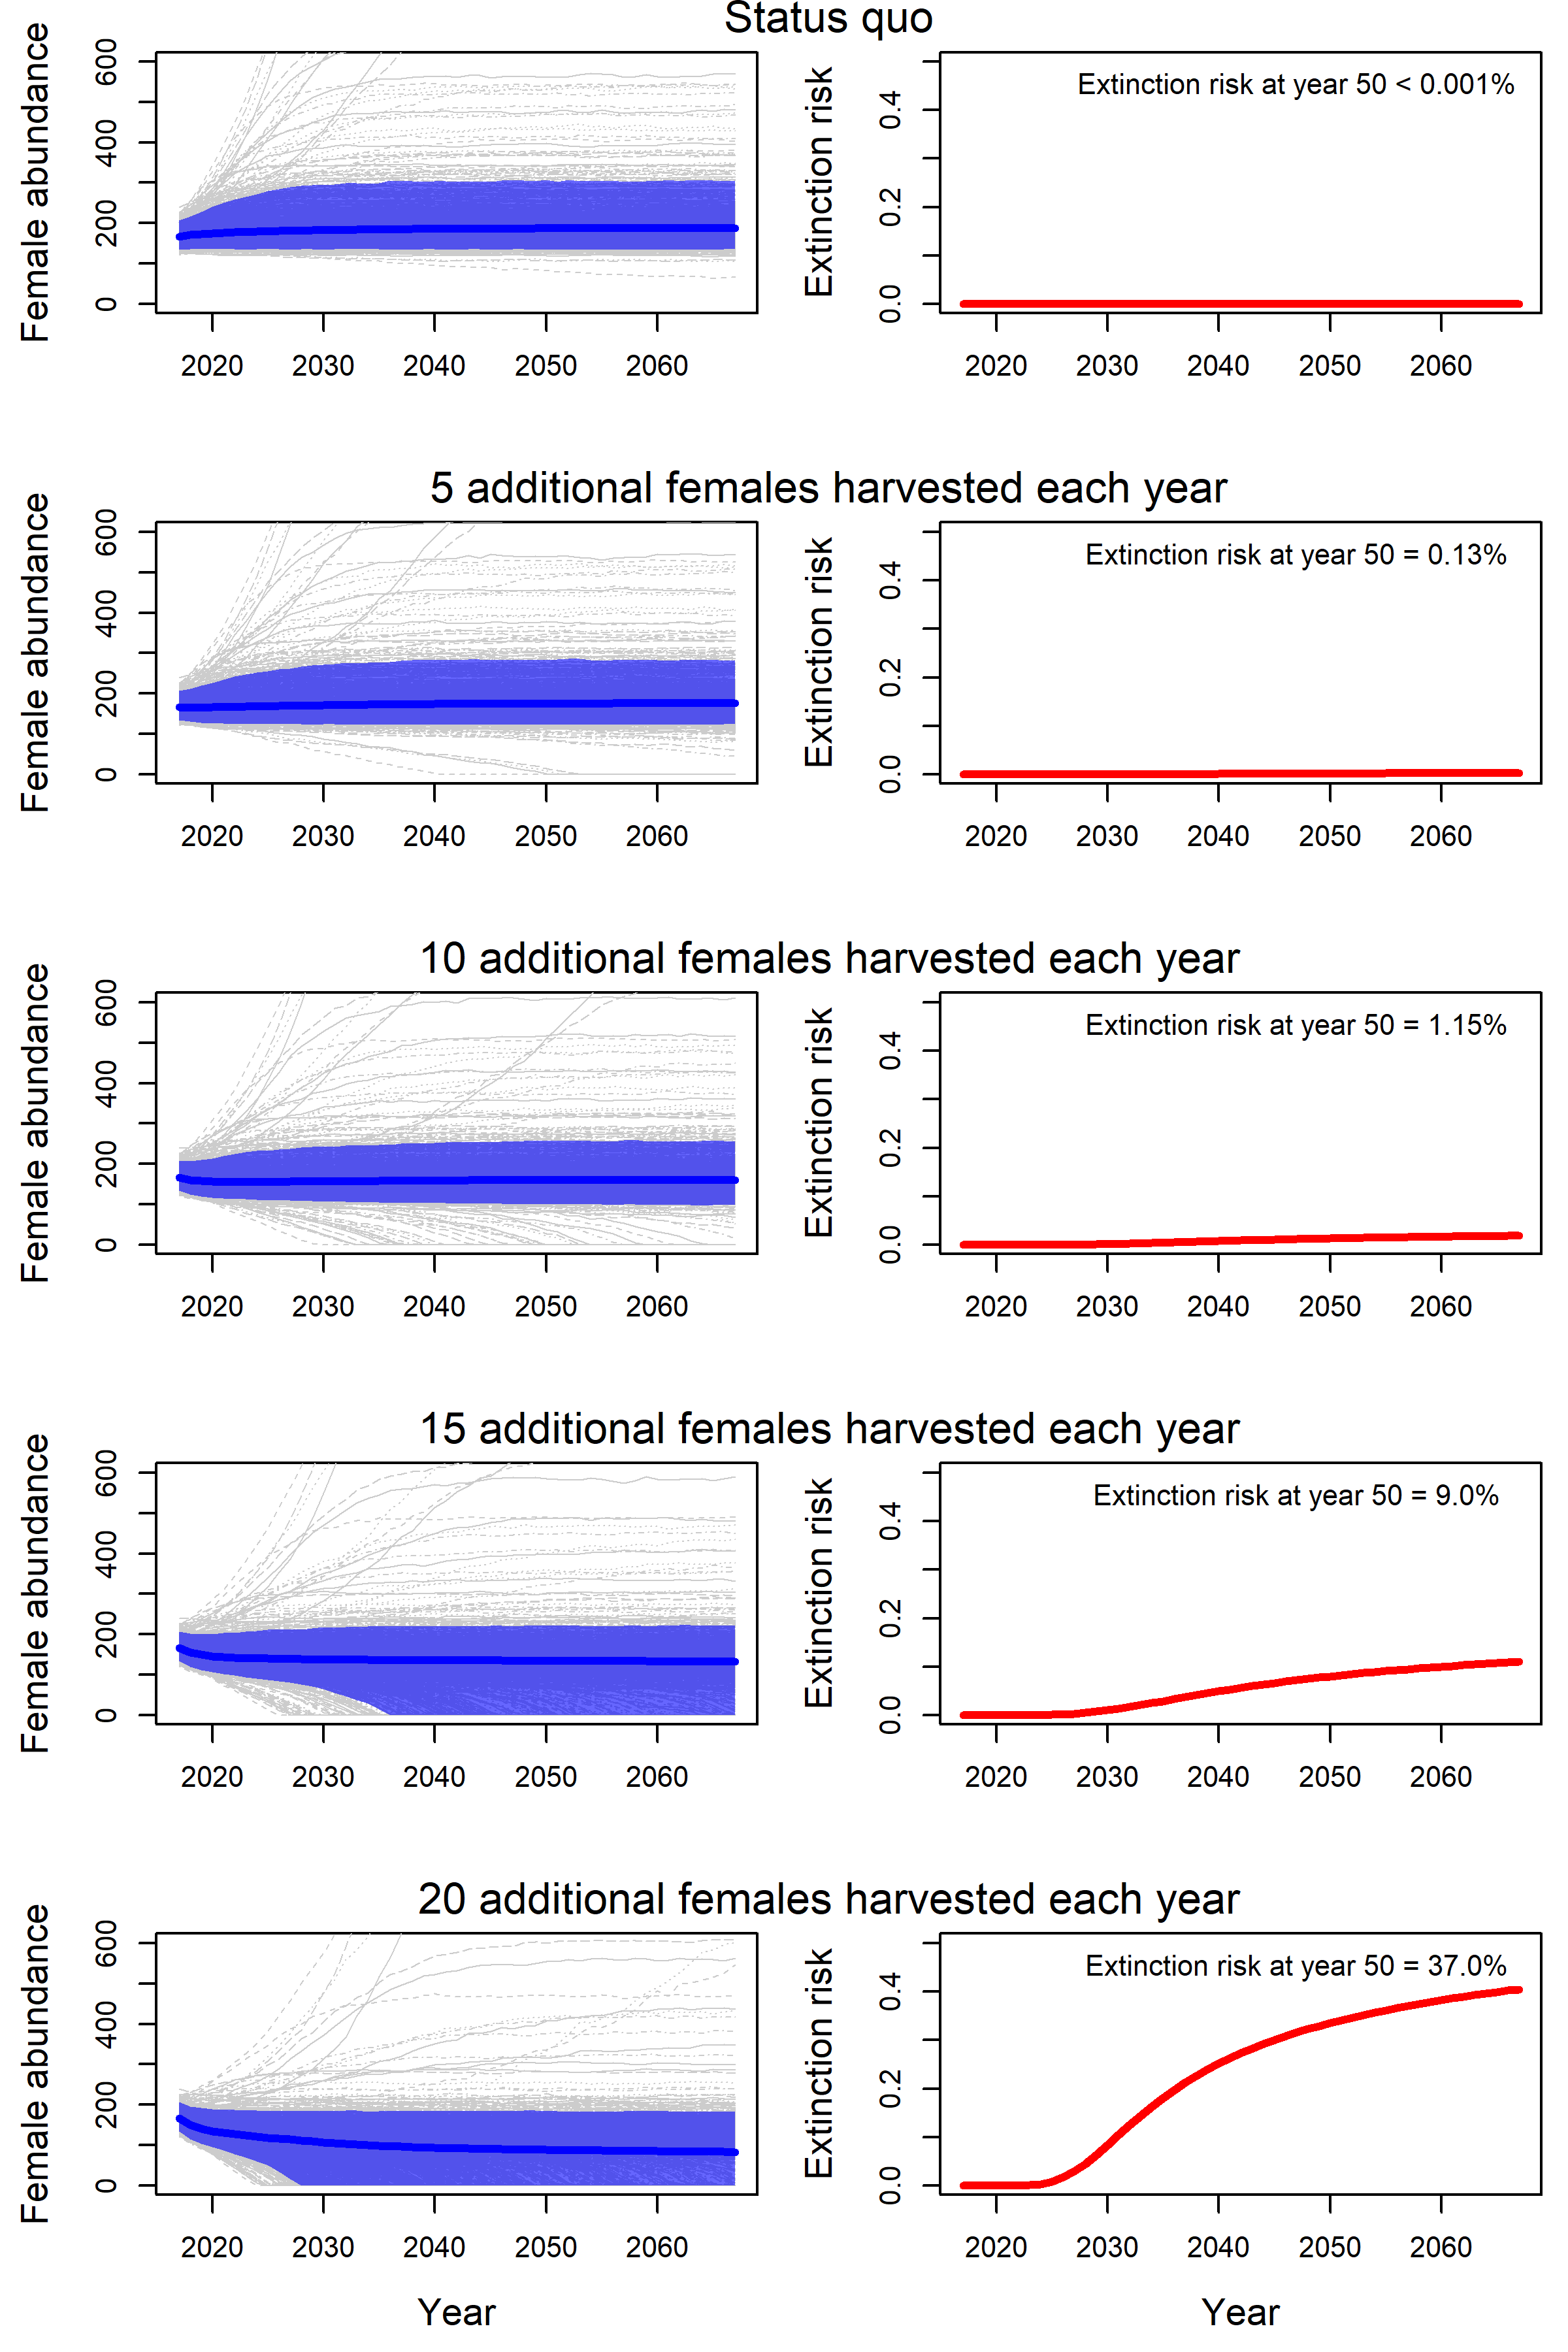
\includegraphics[width=0.45\textwidth]{figs/fig-6_forecasts_h0-h20} \\
\end{frame}




\section{Syllabus}


\begin{frame}
  \frametitle{Books}
  \begin{columns}
    \begin{column}{0.33\textwidth}
      \centering
      AHM vol I\\
      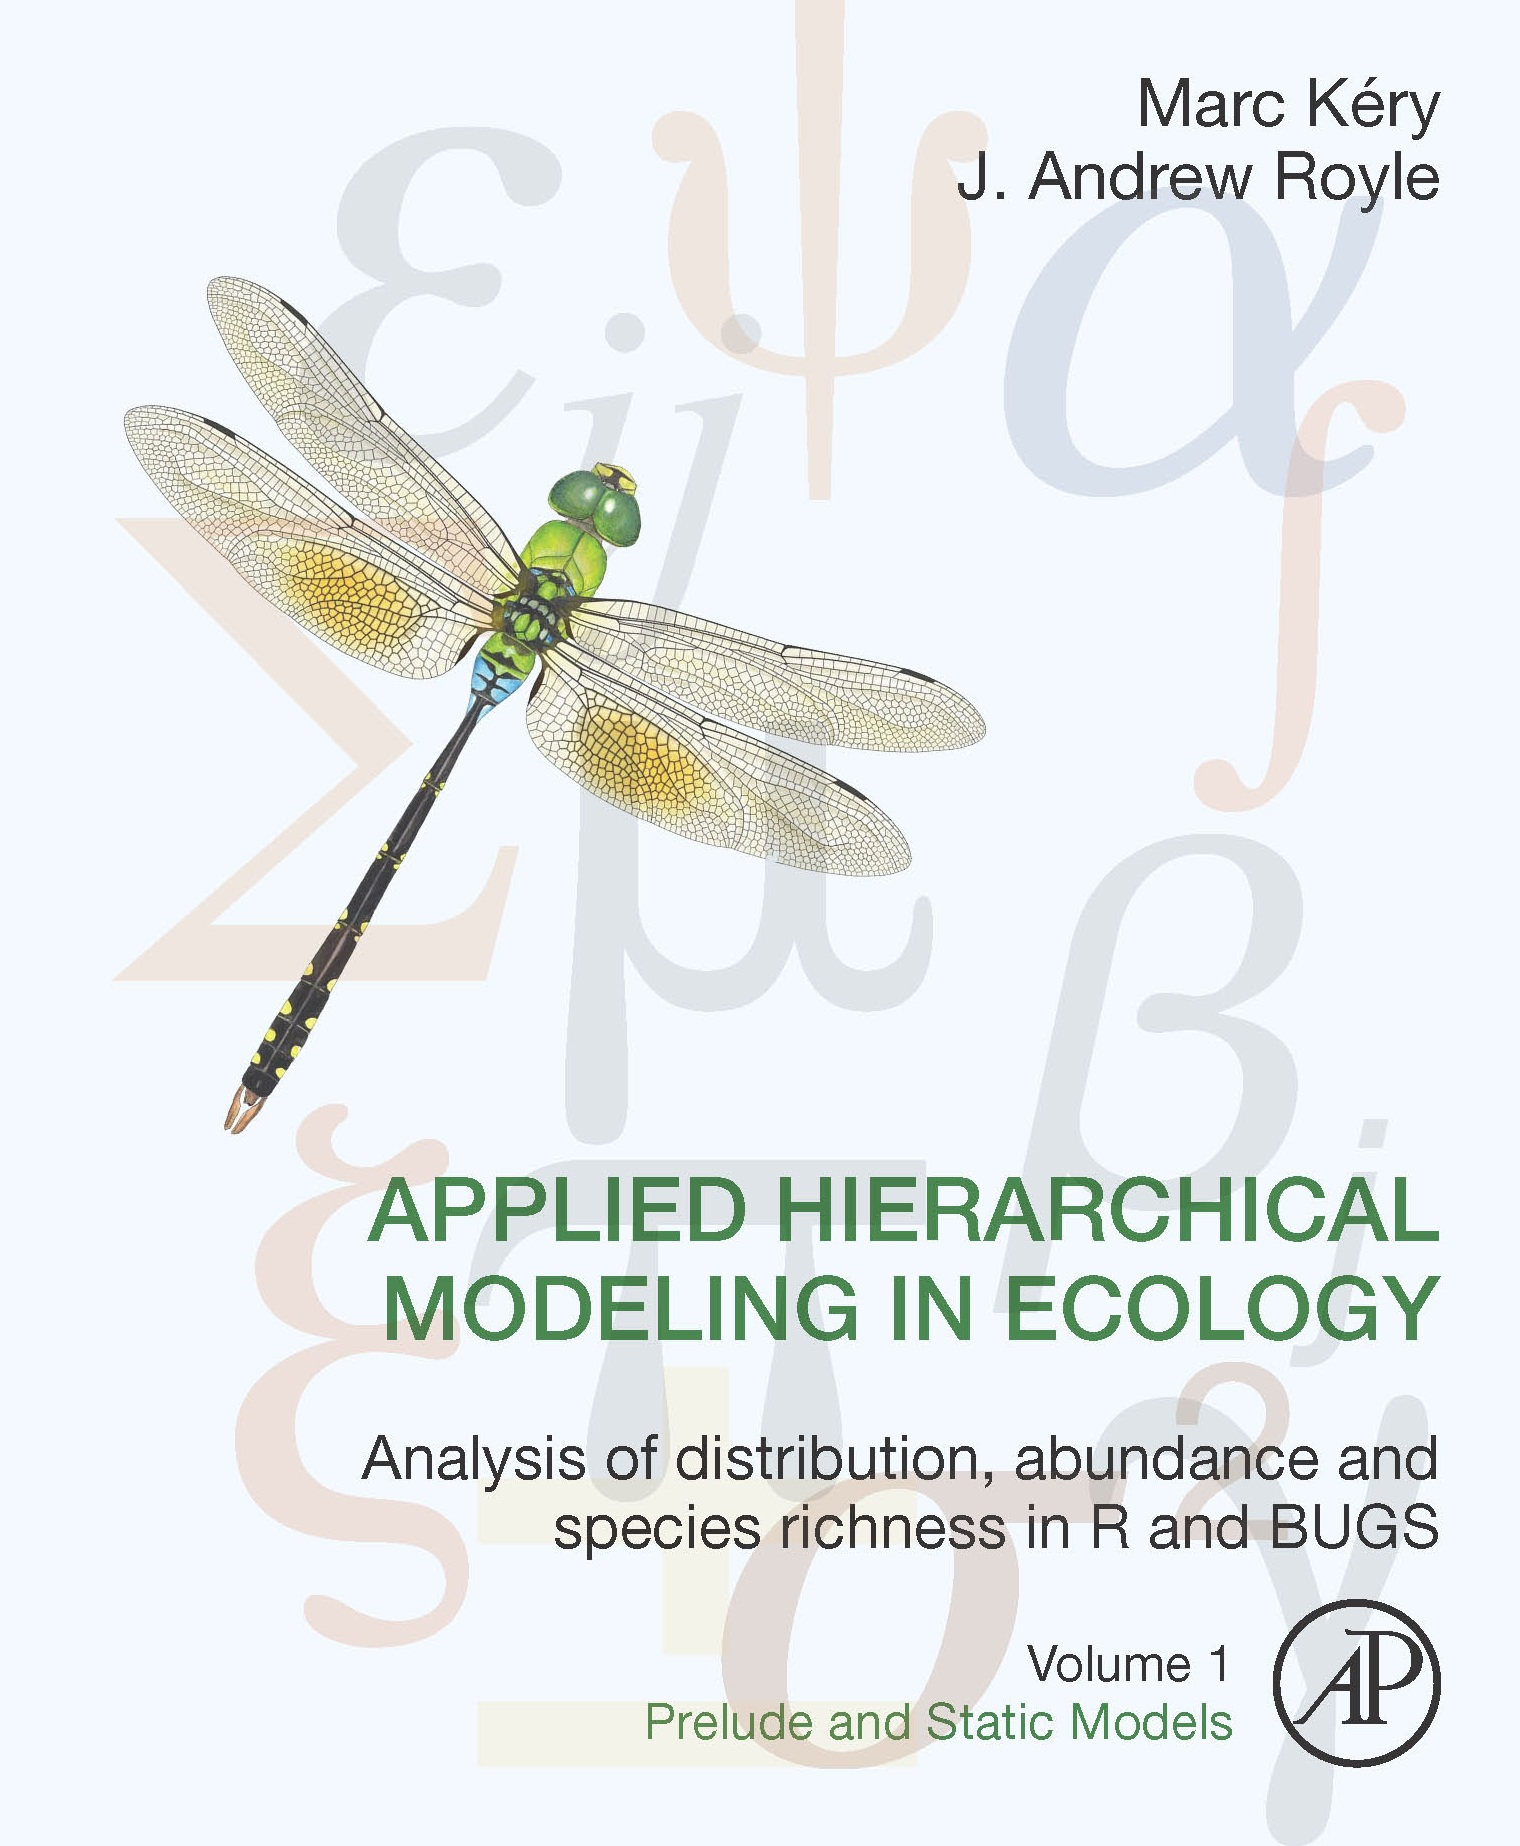
\includegraphics[width=\textwidth]{figs/KeryRoyleBookCover} \\
    \end{column}
    \begin{column}{0.33\textwidth}
      \centering
      AHM vol II\\
      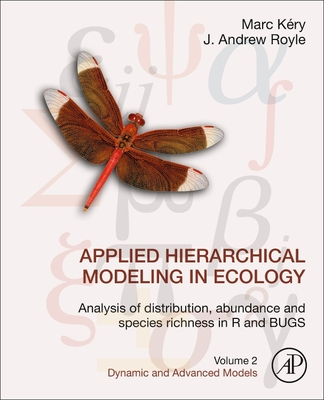
\includegraphics[width=\textwidth]{figs/KeryRoyleBookCoverV2} \\
    \end{column}
    \begin{column}{0.33\textwidth}
      \centering
      SCR \\
      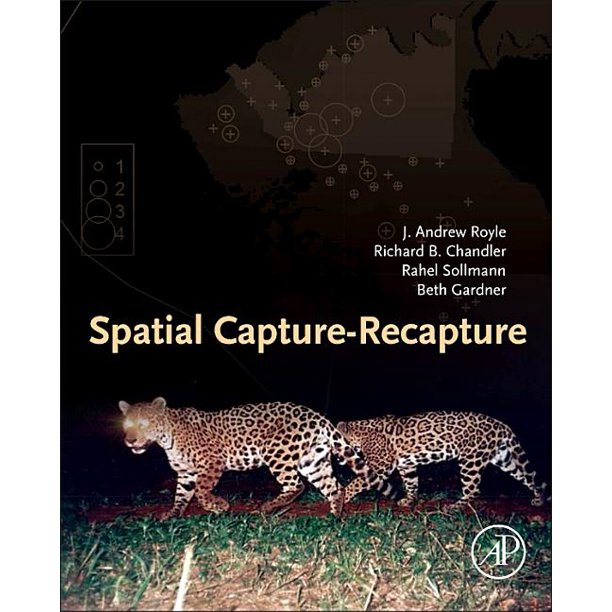
\includegraphics[width=\textwidth,trim=21mm 0mm 21mm 0mm,clip]{figs/SCRcover} \\
    \end{column} 
  \end{columns} 
\end{frame}


\begin{frame}
  \frametitle{Recommended reading}
  \begin{columns}[c]
    \setlength\fboxsep{0pt}
    \begin{column}{0.5\textwidth}
      \centering
      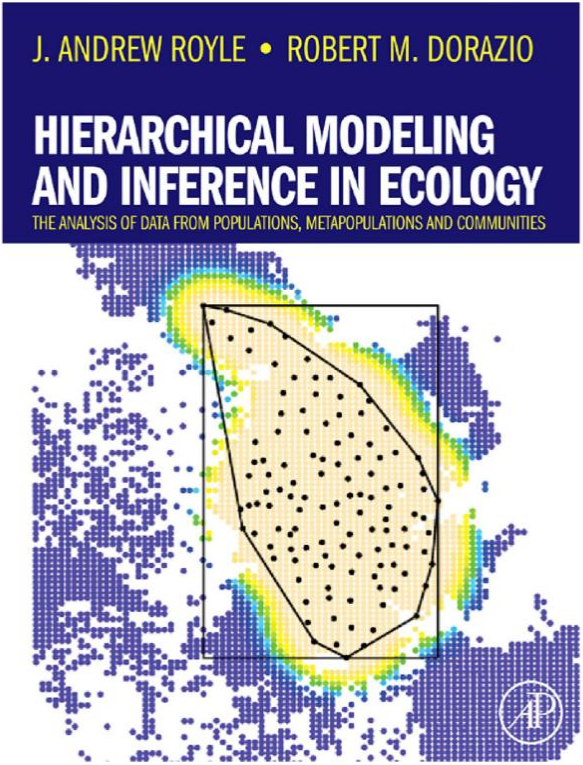
\includegraphics[height=6cm]{figs/RoyleDorazioBookCover} \\
    \end{column}
    \hfill
    \begin{column}{0.5\textwidth}
      \centering
      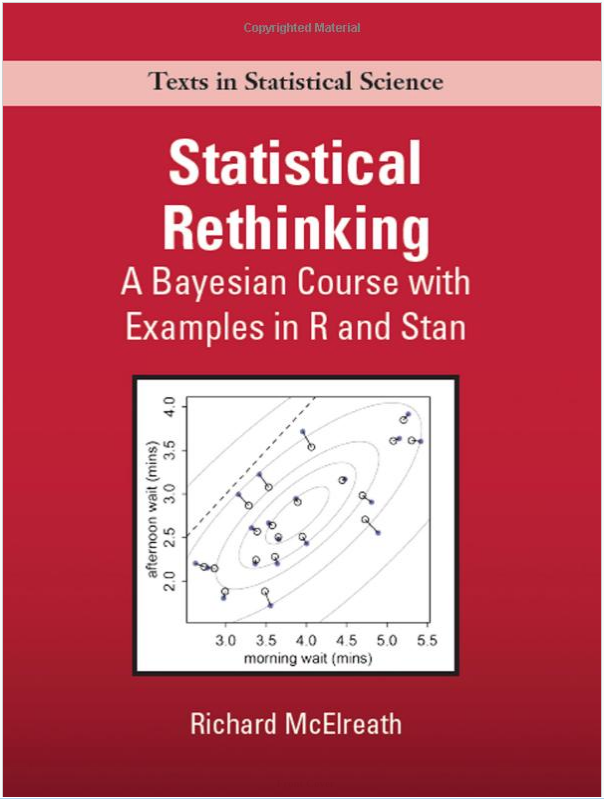
\includegraphics[height=6cm]{figs/McElreathBookCover} \\
    \end{column}
  \end{columns}
\end{frame}



\section{Assignment}


\begin{frame}
  \frametitle{Assignment}
  \large
  Read: Applied Hierarchical Modeling (AHM vol I) front-matter and chapter 1 \\
  \vfill
  Install: \href{https://sourceforge.net/projects/mcmc-jags/files/}{\jags},
  \href{https://www.r-project.org/}{\R}, and the following packages:
  \begin{itemize}
    \tt
    \item unmarked
    \item rjags
    \item jagsUI
  \end{itemize}
\end{frame}





\end{document}
